We refer to the procedure for mapping a cell-centered Cartesian field to a
cell-centered radial array as a lateral ``average''.  We refer to the procedures for mapping
an edge- or cell-centered radial field to an edge- or cell-centered Cartesian grid
as a ``fill''.
\subsubsection{Average}\label{Sec:Average}
For any Cartesian cell-centered field, $\phi$, we define 
$\overline{\phi} = ${\bf Avg}$(\phi)$ as the average over a layer at 
constant radius $r$, $\Omega_H$, as
\begin{equation}
\overline{\phi(r)} = \frac{1}{A(\Omega_H)}\int_{\Omega_H}\phi(r,\xb)d\Omega; \qquad
A(\Omega_H) = \int_{\Omega_H}d\Omega.
\end{equation}
\begin{description}
\item[planar:] 
  This is a straightforward arithmetic average of cells at a particular
  height since the radial cell centers are in alignment with the Cartesian 
  grid cell centers.
\item[spherical:] It can be shown that any Cartesian cell center is a
  radius $\hat r_m = \Delta x\sqrt{\sfrac{3}{4} + 2m}$ from the center of
  the star, where $m \ge 0$ is an integer.  
  For example, the Cartesian cell with coordinates $(i,j,k) = (1,1,1)$ relative
  to the center of the star lies at a distance of $\Delta x\sqrt{\sfrac{3}{4}+6}$
  from the center of the star, corresponding to $m=3$.  The Cartesian cells
  with coordinates $(i,j,k) = (2,0,0), (0,2,0)$, or $(0,0,2)$ relative to
  the center of the star also lie at that same 
  distance.  For the 384$^3$ resolution
  examples in this paper, we have verified that a non-zero set of
  Cartesian cell centers map into each radius $\hat r_m$ until $m$ is 
  large enough to correspond to a radius larger
  than half the width of the computational domain (i.e., the edge of the
  domain, not the corner of the domain).  Figure 
  \ref{Fig:test_average3} shows the number of Cartesian cells that map into each 
  radius $\hat r_m$, which we refer to as the ``hit count'', for a 384$^3$ domain.  
  We use this mapping to help construct the lateral average, using the following steps:
\begin{enumerate}
\item Create an itemized list, $\hat\phi_m$, where each element is
  associated with a radius $\hat r_m = \Delta x\sqrt{\sfrac{3}{4} + 2m}$ from the 
  center of the star.
\item For each $\hat\phi_m$, compute the arithmetic average value of the Cartesian 
  cells whose centers lie at the associated radius.  As an additional 
  element in the itemized list, include the center of the star (corresponding
  to a radius of $r=0$).  Compute this additional value of $\hat\phi$
  at this location using quadratic interpolation with $\hat\phi_0$, $\hat\phi_1$,
  and a homogeneous Neumann condition at $r=0$ as the stencil points.  Note
  that for very large values of $m$, it is possible that no Cartesian cell centers
  exist at a radius $\hat r_m$ (i.e., the hit count is zero).  
  If so, we say that $\hat\phi_m$ has an 
  undefined/invalid value, and we ignore such values for the rest of this procedure.
\item To compute the lateral average, use quadratic interpolation using the 
  value in the itemized list with the closest associated radius, $\hat\phi_k$,
  and the nearest values above and below, $\hat\phi_{k_+}$ and $\hat\phi_{k_-}$,
  using divided differences:
  \begin{equation}
    \overline{\phi(r)} = \hat\phi_{k_-} + \frac{\hat\phi_k-\hat\phi_{k_-}}{\hat r_k-\hat r_{k_-}}(r-\hat r_{k_-}) + \frac{\frac{\hat\phi_{k_+}-\hat\phi_k}{\hat r_{k_+}-\hat r_k}-\frac{\hat\phi_k-\hat\phi_{k_-}}{\hat r_k-\hat r_{k_-}}}{\hat r_{k_+}-\hat r_{k_-}}(r-\hat r_{k_-})(r-\hat r_k)\nonumber,
  \end{equation}
  where $\hat r_{k_-}$, $\hat r_k$, and $\hat r_{k_+}$ are the three radii
  associated with $\hat\phi_{k_-}$, $\hat\phi_k$, and  $\hat\phi_{k_+}$.
  Finally, constrain $\overline{\phi(r)}$ to lie within the range of
  $\hat\phi_{k_-}$, $\hat\phi_k$, and $\hat\phi_{k_+}$ so as to not introduce
  any new maxima or minima.
\end{enumerate}
  In \S \ref{Sec:Mapping Test}, we show the improvement of this averaging procedure 
  over the Paper IV procedure.
\end{description}
%%%%%%%%%%%%%%%%%%%%%%%%%%%%%%%%%
\begin{figure}[h]
\centering
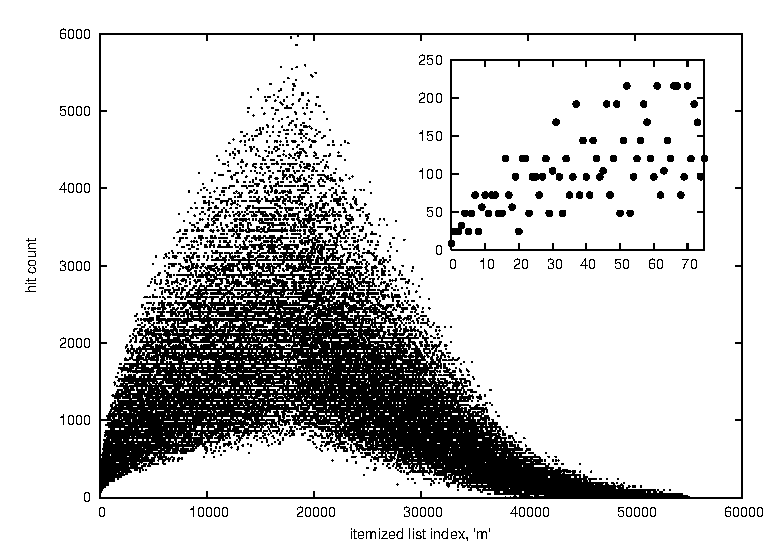
\includegraphics{\radbasefigpath/test_average3}
\caption{\label{Fig:test_average3}
The number of Cartesian cells whose centers lie
at a radius $\hat r_m$ (i.e., the ``hit count'') for a 384$^3$ domain vs. the
itemized list index, $m$.  
Indices $m<18,432$ correspond to locations within half the width 
of the computational domain.  A non-zero set of Cartesian cell centers maps 
into the radius associated with every $m\le 37,912$, which corresponds to 
approximately 0.72 times the width of the computational domain.  The inset plot
is a zoom-in of the innermost 75 values of $m$.}
\end{figure}
%%%%%%%%%%%%%%%%%%%%%%%%%%%%%%%%%
\subsubsection{Fill}\label{Sec:Fill}
There are four different mappings from a 1D radial array to the 3D Cartesian grid;
below we describe the procedures for planar and spherical geometries separately.
\begin{description}
\item[planar:]
\end{description}
\begin{enumerate}
\item To map a cell-centered radial array onto Cartesian cell centers,
  we use direct-injection since the radial cell centers are in
  alignment with the Cartesian cell centers. 
\item To map an edge-centered radial array onto Cartesian 
  cell centers, we average the two nearest radial edge-centered values.
\item To map a cell-centered radial array onto Cartesian edges with normal in 
  the radial direction, we use 4th order spatial interpolation:
\begin{equation}
\phi_{i,j,k+\myhalf} = \frac{7}{12}(\phi_{j}+\phi_{j+1}) - \frac{1}{12}(\phi_{j-1}+\phi_{j+2}).
\end{equation}
  We constrain $\phi_{i,j,k+\myhalf}$ to lie between the interpolated values, and 
  lower the order of interpolation near domain boundaries.  For the 
  Cartesian edges transverse to the base state direction, we use direct-injection 
  since the radial cell centers are in alignment with these 
  Cartesian edges.
\item To map an edge-centered radial array onto Cartesian edges, 
  we use direct-injection on Cartesian edges normal to the base state direction
  since the radial edges are in alignment with these Cartesian edges.  
  For the remaining Cartesian edges, we average the two nearest radial 
  edge-centered values.
\end{enumerate}
\begin{description}
\item[spherical:] 
\end{description}
\begin{enumerate}
\item To map a cell-centered radial array onto Cartesian cell centers,
      we use quadratic interpolation from the nearest 
      three radial cell centers (see Figure \ref{Fig:fill}a).
      This is a departure from Paper IV, in which we used 
      piecewise constant interpolation.  
\item To map an edge-centered radial array onto Cartesian cell centers, 
      we use linear interpolation from the nearest two points
      (see Figure \ref{Fig:fill}b).
\item To map a cell-centered radial array onto Cartesian edges,
      we first map the radial array onto Cartesian cell centers (see 1.), 
      then average the two neighboring centers to obtain the Cartesian edge values
      (see Figure \ref{Fig:fill}c).
\item To map an edge-centered radial array onto Cartesian edges,
      we first map the radial array onto Cartesian cell centers (see 2.), 
      then average the two neighboring centers to obtain the Cartesian edge values
      (see Figure \ref{Fig:fill}c).
\end{enumerate}

%%%%%%%%%%%%%%%%%%%%%%%%%%%%%%%%%
\begin{figure}[tpb]
\centering
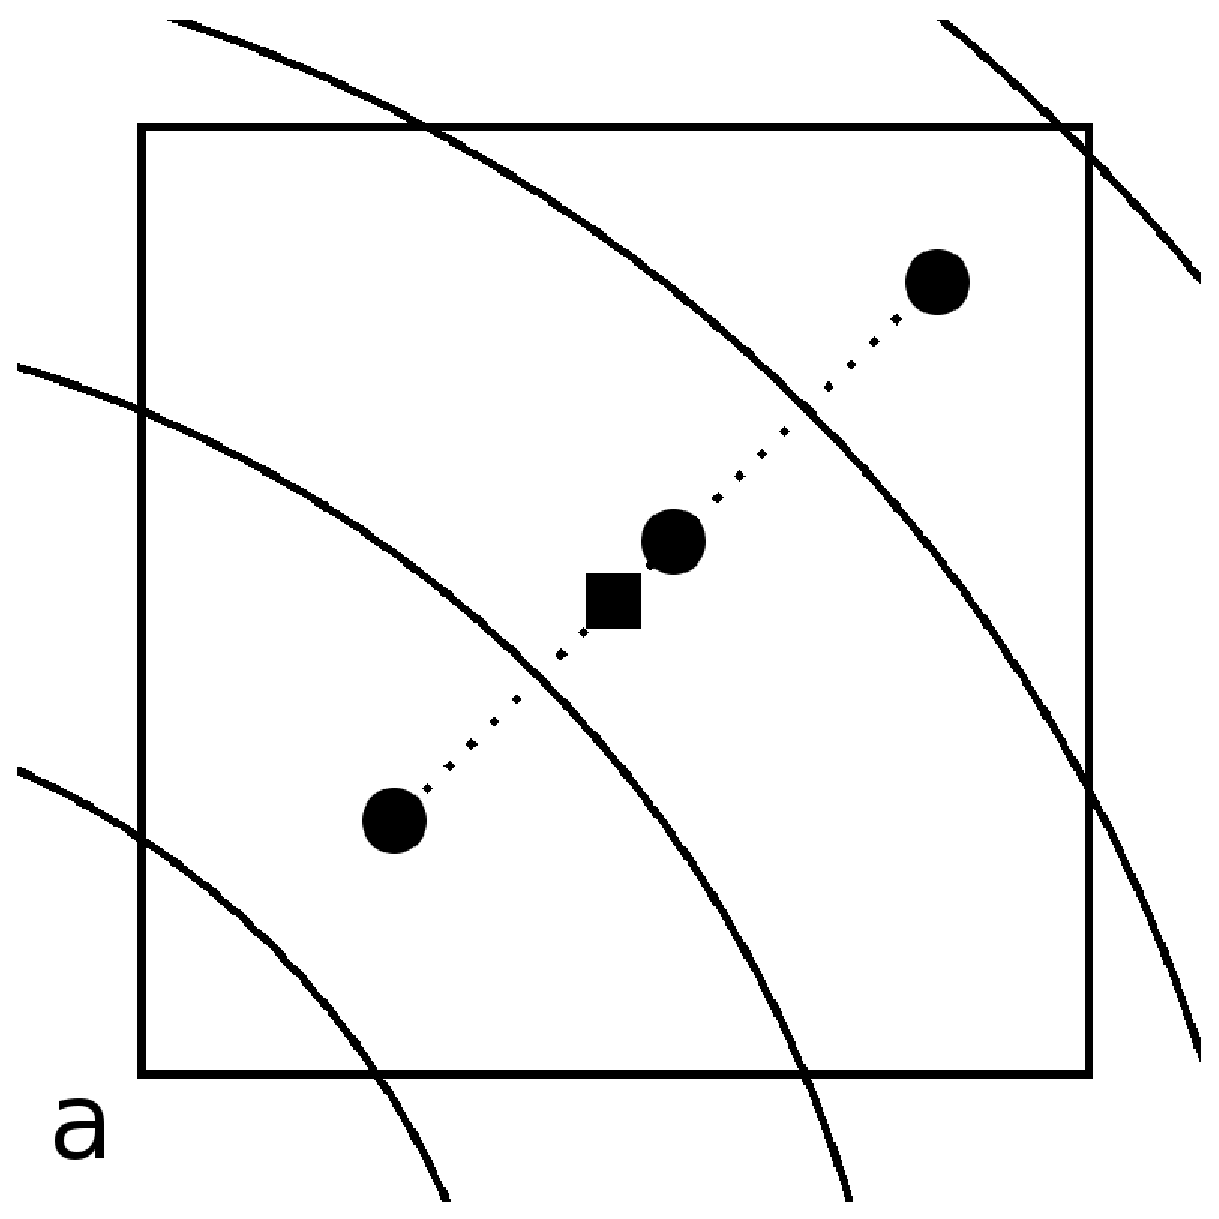
\includegraphics[width=1.75in]{\radbasefigpath/fill1}\hspace{0.1in}
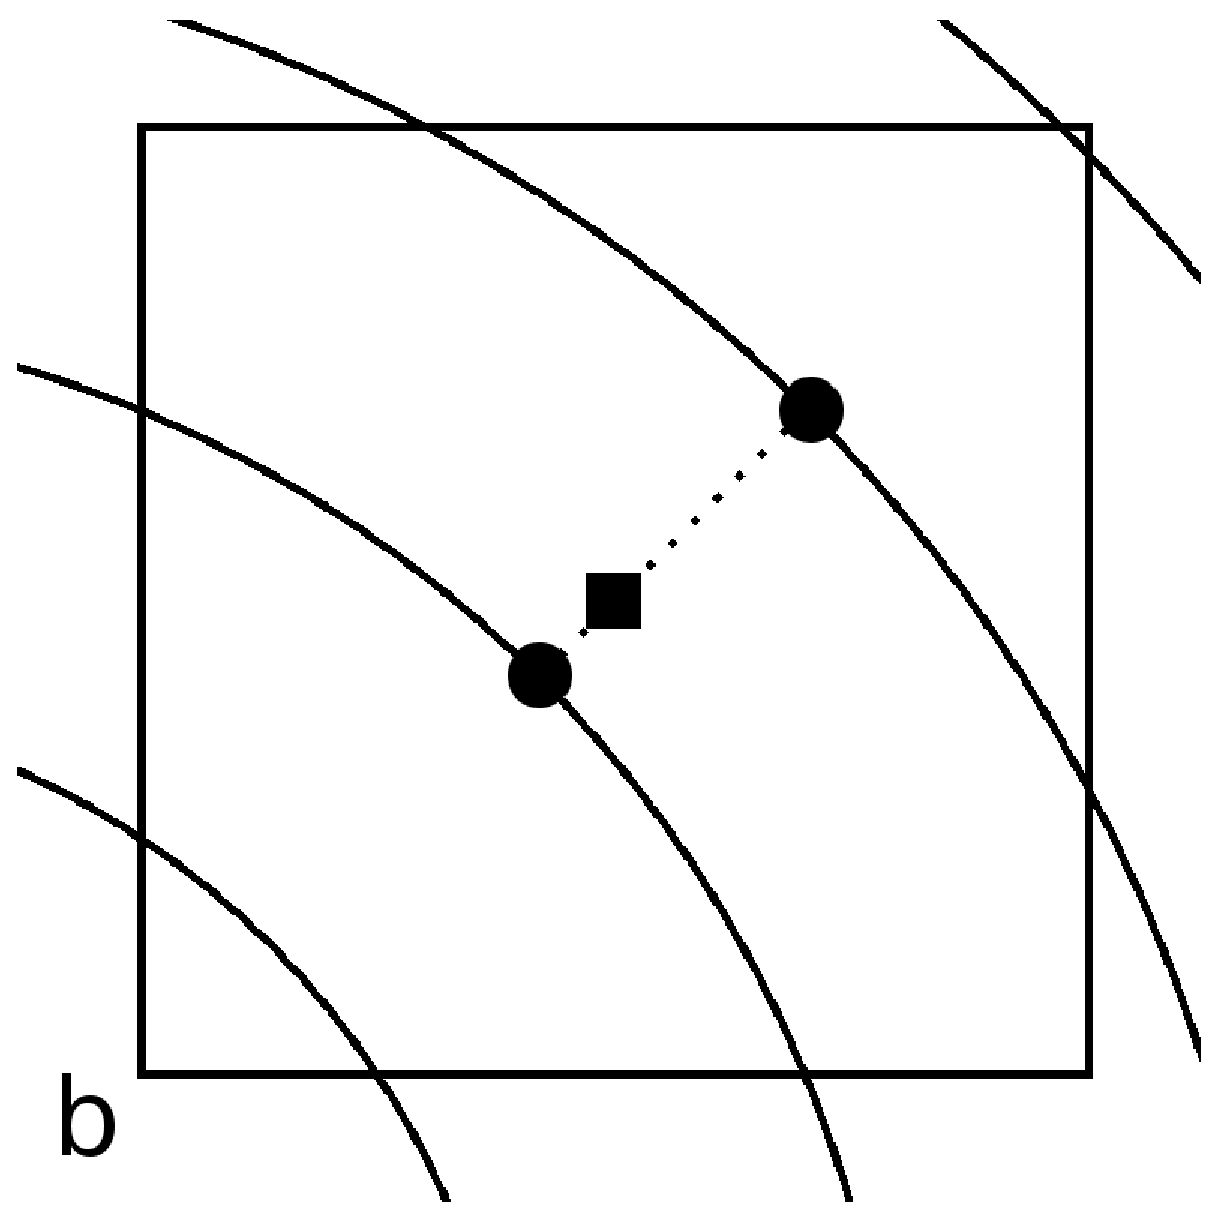
\includegraphics[width=1.75in]{\radbasefigpath/fill2}\hspace{0.1in}
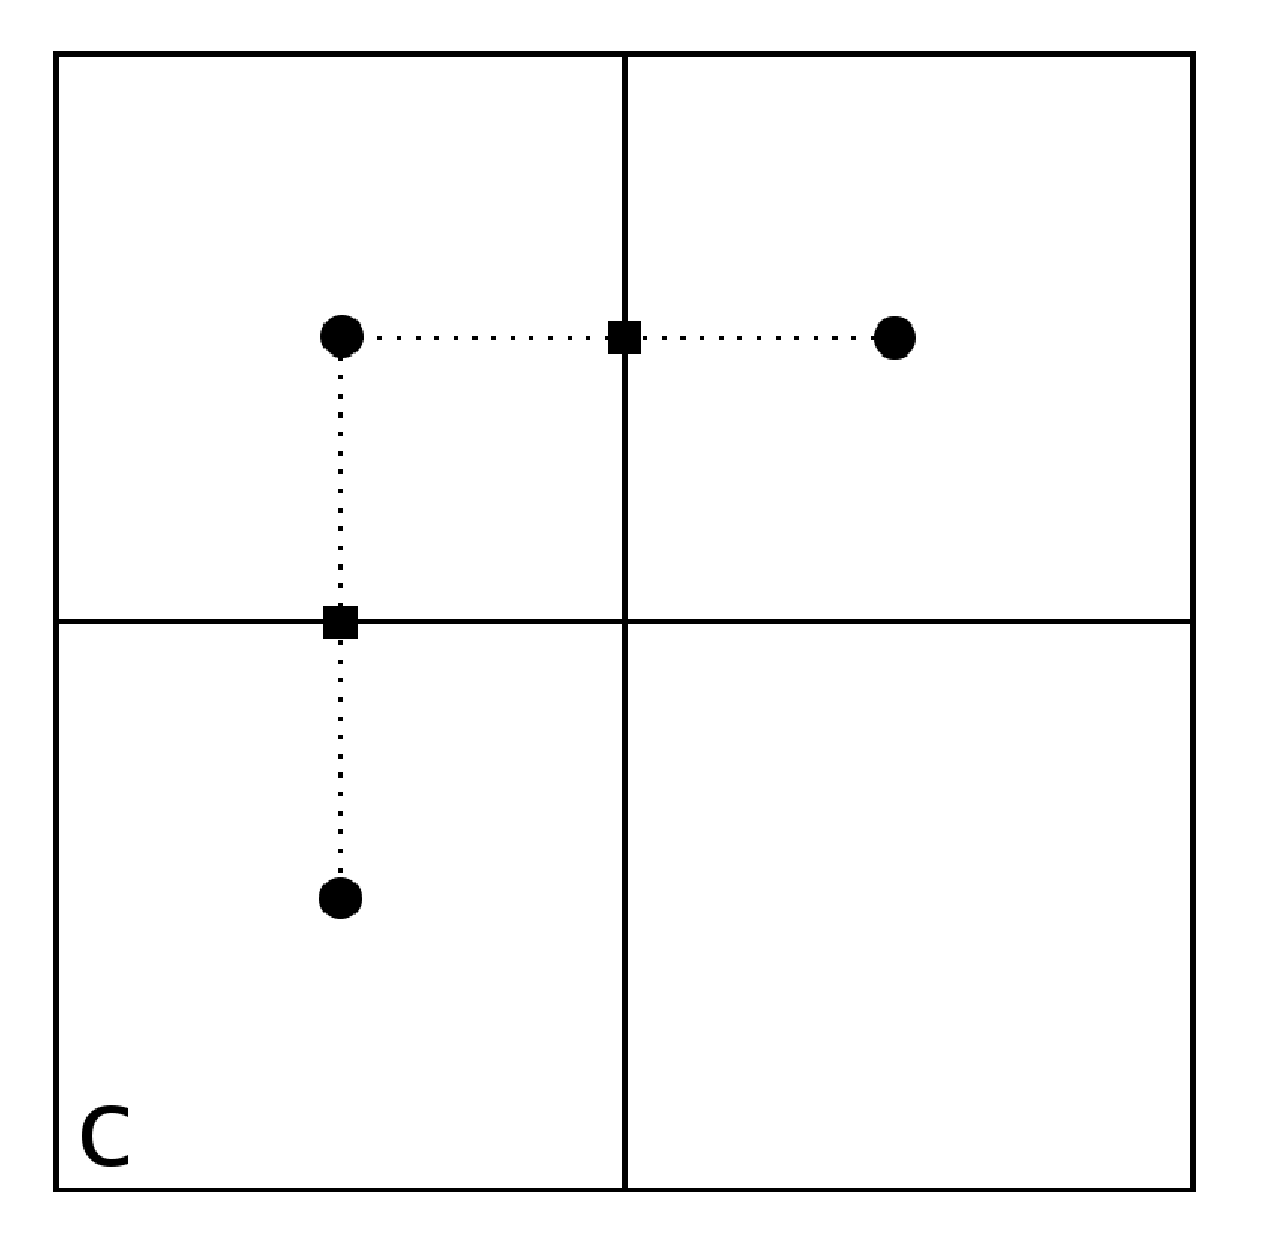
\includegraphics[width=1.75in]{\radbasefigpath/fill3}
\caption{\label{Fig:fill} Illustrations of the fill operation for
  spherical geometry.  (a) To fill the Cartesian cell center (fill
  type 1), represented by the square, from radial cell-centered data,
  represented by the circles, we use quadratic interpolation from the
  nearest three points.  (b) To fill the Cartesian cell center
  (fill type 2), represented by the square, from radial edge-centered
  data, represented by the circles, we use linear interpolation from
  the nearest two points. (c) To fill a Cartesian edge (fill
  types 3 and 4), represented by the squares, first fill the 
  Cartesian cell centers, represented by the circles, then average
  the two neighboring cell centers.}
\end{figure}
%%%%%%%%%%%%%%%%%%%%%%%%%%%%%%%%%
